\chapter{Resultater}

\section{Det færdige system}
- Kamera


\section{Koncept analyse}
hmm...
 
\section{Kravspecifikation og accepttest}
\label{subsec:krav}
For at vise at der er brugt de beskrevne metoder ovenfor, er der valgt at tage eksempler med i rapporten. %for at eftervise de fire udviklingsfaser projektet har været i gennem.

\subsection{Aktør beskrivelse}
Systemets primære aktør er operatøren, som står for påfyldning af celler, start og stop af sorteringsprocessen. Operatøren har mulighed for at interagere med systemet via en grafisk brugergrænseflade. Systemets sekundære aktør er kameraet og PC’ens filsystem. Kameraet er systemets interface til detektion af de Langerhanske øer. Filsystemet er hvor der løbende gemmes en log over sorteringsprocessen.

\subsection{Use Case Diagram}
I Use Case diagrammet (figur: \ref{fig:usecase}) er der vist, hvilke use cases systemet \textit{The Cell Collector} består af. Yderligere er det vist, hvilke aktører der initiere de enkelte use cases. På venstre side er systemets primære aktør \textit{operatøren} vist, mens systemets sekundære aktører \textit{kamera} og \textit{database} er placeret i højre side. 

\begin{figure}[H]
	\centering
	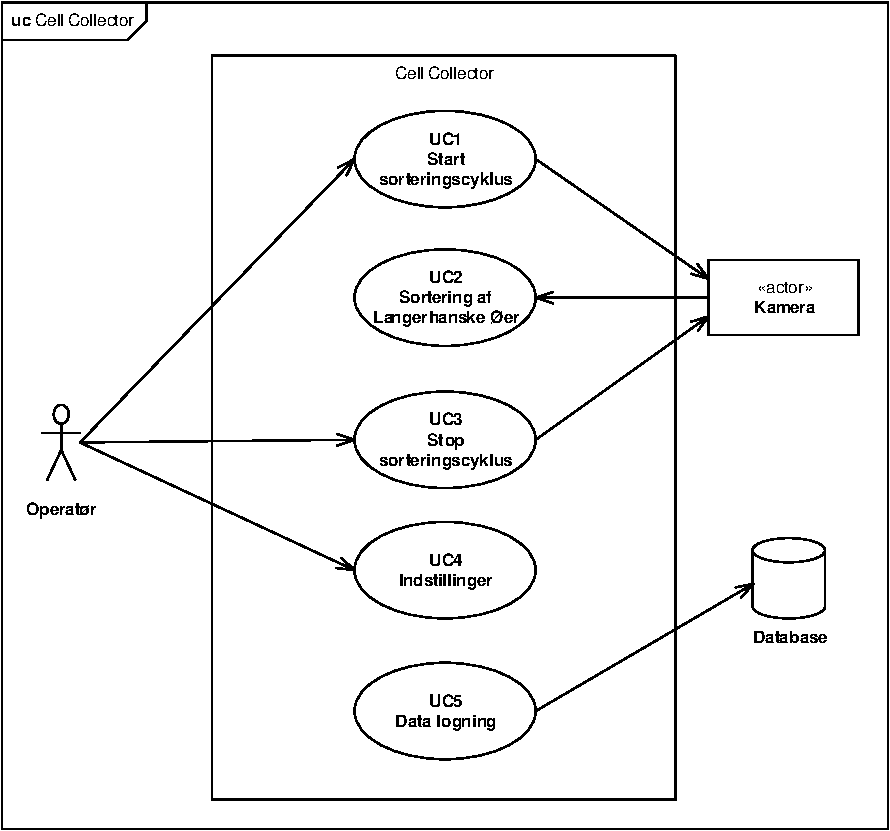
\includegraphics[width=1\textwidth]{billeder/UC_CellCollector.pdf}
	\caption{Use Case diagram for The Cell Collector}
	\label{fig:usecase}
\end{figure}
Efter use case diagrammet var færdigt, blev der udarbejdet fully dressed use cases som kan ses på nedenstående tabel. Tabellen beskriver normalforløbet og undtagelser for \textit{Start sorteringscyklus}, som er den første use case på diagrammet. 
\newpage 

\label{uc:1}
\begin{center}
		\begin{longtable}{ | m{4cm} | m{8cm}| } 
			\hline
			Mål & Start sorteringscyklus \\ 
			\hline
			Initiering &  Use casen initieres af operatøren\\
			\hline
			Aktør & 
			Primær: Operatør
			
			 Sekundær: Kamera			  \\ 
			\hline
			Startbetingelser & The Cell Collector programmet er startet på computeren \\ 
			\hline	
			Slutbetingelser ved succes & Systemet starter med sorteringen af Langerhanske øer \\
			\hline
			Slutbetingelser ved undtagelse & N/A \\
			\hline
			Normalforløb & \begin{enumerate}
				%\setlength\itemsep{0cm} % Decrease line distance
				\item Operatør fylder celleopløsningsbeholderen
				\item Celleopløsningsbeholderen er fyldt
				\item Operatør starter sorteringscyklus ved at klikke på [Start]
				\subitem [Undtagelse 1: Wastebeholder er fyldt] 
				\item Systemet initialiserer Arduinoen
				\subitem [Undtagelse 2: Ingen forbindelse til Arduino]
				\item Systemet kontrollerer celleopløsningsbeholderen ved at konvertere spændingen (\SI{}{\volt})  til \SI{}{\milli\litre}, og vise beholderens indhold (\SI{}{\milli\litre}) på GUI
				\item Systemet initialiserer kameraet
				\subitem [Undtagelse 3: Kameraet initialiserer ikke]
				\item Systemet tænder for kamera lyset
				\item Systemet tænder for pumpen
				
			\end{enumerate} \\ 
			\hline
			Undtagelser & [Undtagelse 1: Wastebeholder er fyldt] 
			
			\begin{enumerate}
			\item Systembesked: Tøm venligst Wastebeholder før start
			\item Operatøren trykker “OK”
			\item Systemet fortsætter opstartprocessen
			\end{enumerate} 
			
			[Undtagelse 2: Ingen forbindelse til Arduino]
			
			\begin{enumerate}
			\item 1.	Systembesked: Ingen forbindelse til Arduino, kontrollér forbindelser.
			\end{enumerate} 
	
			[Undtagelse 3: Kameraet initialiseres ikke]
			
			\begin{enumerate}
			\item System fejlmeddelse: Kameraet er ikke initialiseret:
			\item Genstart initialisering af Kameraet
			\end{enumerate} \\
			\hline
		\end{longtable}
	\end{center}

Efter at normalforløbet og undtagelserne er defineret, blev acceptesten lavet for den givne use case. Til hvert punkt i normalforløbet er der forberedt en test, som indeholder et krav nr, handling dvs det der skal gøres for at starte testen. Derudover er der forventet resultat, som skal ske for at testen kan godkendes. Testmetode beskriver hvordan testen skal udføres og hvordan den godkendes.

\begin{center}
		\begin{longtable}{ | m{4cm}| m{8.5cm}|} 
			\hline
			\textbf{Krav nr.} & 1.1 \& 1.2    \\ 
			\hline
			\textbf{Handling} &  Operatør fylder celle-opløsnings-beholderen   \\
			\hline
			\textbf{Forventet resultat} &  Celle opløsningsbeholderen er fyldt  \\
			\hline
			\textbf{Testmetode}  &  Celle opløsningsbeholderen fyldes med væske  \\
			\hline
			\textbf{Resultat}  &    \\
			\hline
			\textbf{Angiv godkendelse} &     \\
			\hline
			\textbf{Initialer} &     \\
			\hline
			\textbf{Dato} &    \\
			\hline
		\end{longtable}
	\end{center}
	
	
	\begin{center}
		\begin{longtable}{ | m{4cm}| m{8.5cm}|} 
			\hline
			\textbf{Krav nr.} & 1.3    \\ 
			\hline
			\textbf{Handling} &  Operatør starter sorteringscyklus ved at klikke på [Start]  \\
			\hline
			\textbf{Forventet resultat} &  Opstarts processen i gang sættes.  \\
			\hline
			\textbf{Testmetode}  & Knappen [Start] trykkes, observeres ved tekstboks på GUI, med teksten \textit{systemet starter op}.   \\
			\hline
			\textbf{Resultat}  &    \\
			\hline
			\textbf{Angiv godkendelse} &     \\
			\hline
			\textbf{Initialer} &     \\
			\hline
			\textbf{Dato} &    \\
			\hline
		\end{longtable}
	\end{center}
	
	\begin{center}
		\begin{longtable}{ | m{4cm}| m{8.5cm}|} 
			\hline
			\textbf{Krav nr.} & 1.4    \\ 
			\hline
			\textbf{Handling} &  Systemet initialisere Arduinoen   \\
			\hline
			\textbf{Forventet resultat} &  Arduino initialiseret signal modtages og gives til GUI  \\
			\hline
			\textbf{Testmetode}  & Det observeres på GUI at Arduinoen er initialiseret, i en tekstboks med testen \textit{Arduino er initialiseret}.   \\
			\hline
			\textbf{Resultat}  &    \\
			\hline
			\textbf{Angiv godkendelse} &     \\
			\hline
			\textbf{Initialer} &     \\
			\hline
			\textbf{Dato} &    \\
			\hline
		\end{longtable}
	\end{center}
	
	\begin{center}
		\begin{longtable}{ | m{4cm}| m{8.5cm}|} 
			\hline
			\textbf{Krav nr.} & 1.5    \\ 
			\hline
			\textbf{Handling} &  Systemet kontrollerer celle-opløsnings-beholderen  \\
			\hline
			\textbf{Forventet resultat} &  Antal ml i celleopløsningsbeholderen vises på GUI.  \\
			\hline
			\textbf{Testmetode}  & Der hældes 100 ml i celleopløsningsbeholderen, det observeres på GUI om der vises 100 ml $\pm$ 10 ml   \\
			\hline			
			\textbf{Resultat}  &    \\
			\hline
			\textbf{Angiv godkendelse} &     \\
			\hline
			\textbf{Initialer} &     \\
			\hline
			\textbf{Dato} &    \\
			\hline
		\end{longtable}
	\end{center}	
	
Resten af acceptesten for use case 1 kan ses i projektdokumentationen \fxnote{hvordan skal der refereres her til ?} 

\section{Design}
\label{subsec:design}
I dette afsnit er der givet et eksempel på hvordan projektet er gået fra krav til en måde at løse projektet på. Der er blandt andet brugt BDD, IBD, flowchart samt sekvensdiagrammer til at beskrive funktioner og sammenhænge i projektet. 

\subsection{BDD og IBD for hardware}
Nedenstående BDD \ref{fig:bdd_Hardware} giver et overordnet overblik i, hvad \textit{The cell collector} indeholder af hardware elementer. Hierarkiet starter øverst med \textit{The cell collector}, som indeholder tre mindre hardware dele. Styreenheden der er defineret som en Arduino, den indeholder de elementer der bl.a. motordriveren. Motordriveren indeholder yderligere to dele, som den styrer. Det vil sige at pumpen og ventilen bliver styret i gennem motordriveren. Udover styreenheden er der også ikke elektriske dele, som beholdere og førringsveje til opløsningen med langerhanske øer. Den tredje underblok til \textit{The cell collector} er kameraet.

\begin{figure}[H]
	\centering
	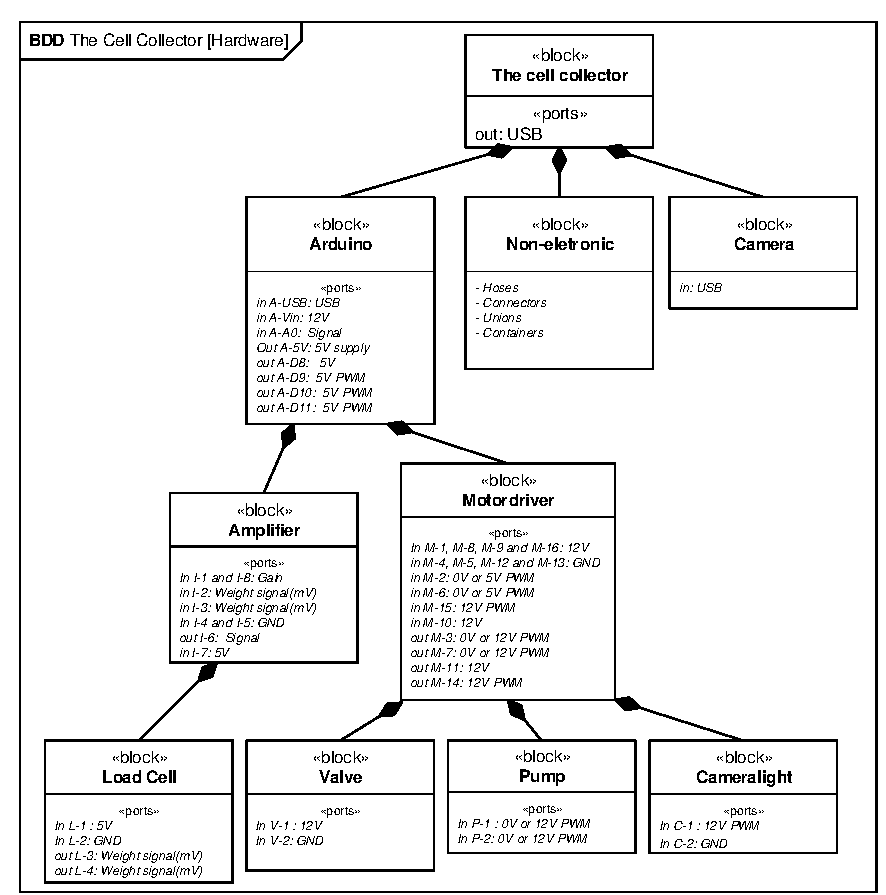
\includegraphics[width=1\textwidth]{pdf/BDD_Hardware.pdf}
	\caption{BDD - Cell Collector [Hardware]}
	\label{fig:bdd_Hardware}
\end{figure}

Nedenstående IBD \ref{fig:ibd_Hardware} beskriver mere præcist, hvordan de forskellige komponenter interagerer med hinanden på. Diagrammet er brugt til, at der tidligt i udviklingsforløbet bliver defineret hvilke spændinger og signaltyper systemet skal indeholde. Systemet skal indeholde bestemte typer for, at kunne kommunikere med de interne dele.


\begin{figure}[H]
	\centering
	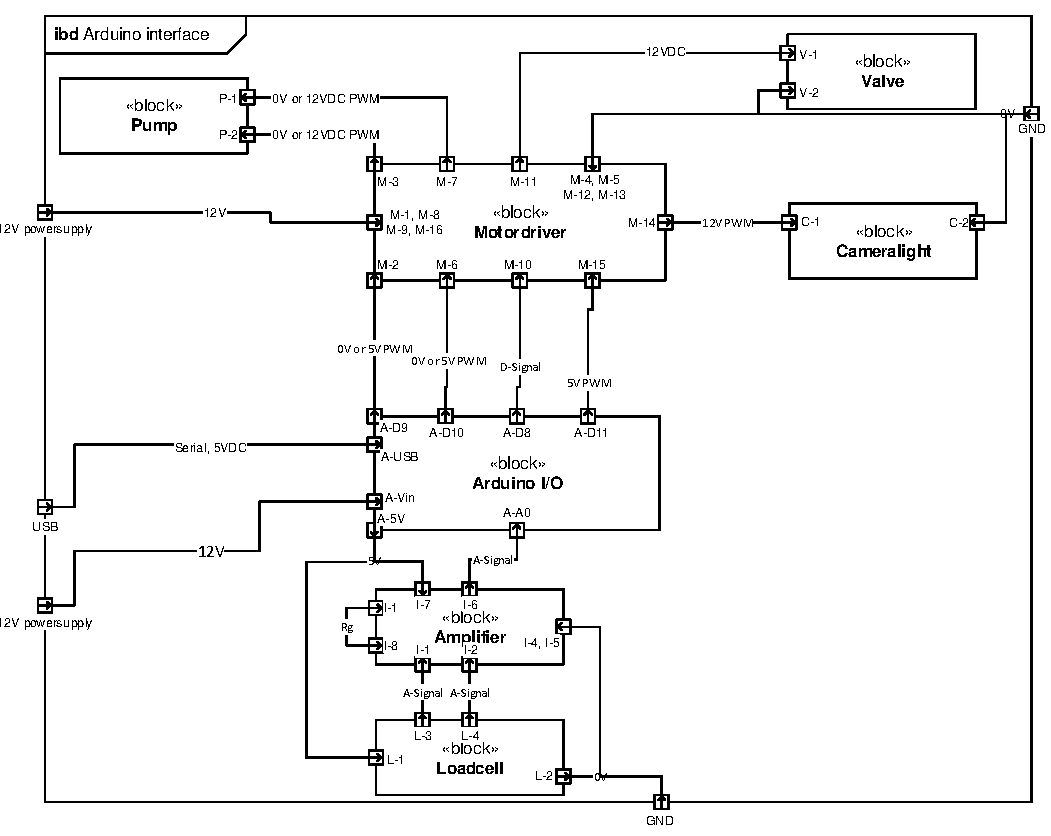
\includegraphics[width=1\textwidth]{pdf/IBD_Hardware(Arduino).pdf}
	\caption{IBD - Cell Collector [Hardware]}
	\label{fig:ibd_Hardware}
\end{figure}

Til ovenstående diagrammer er der udarbejdet tabeller som beskriver signalerne og de enkelte blokke. \fxnote{reference til projektdokumentation}

Ydermere kan der ses specifikationerne for vægtcellen er stillet op og hvilke overvejelser der er gjort ved denne komponent.
\subsection{Vægtcelle}
\label{subsec:loadcell}
Vægtcellen skal bruges til at kontrollere om, der er væske i celleopløsningsbeholderen.

\textbf{Specifikationer for Vægtcelle[\citet{DH7}]:} 
\begin{center}
		\begin{longtable}{ | m{6.5cm} | m{6.5cm}| } 
			\hline
			\textbf{Specifikation} &\textbf{Værdi} \\ 
			\hline
			\textbf{Max belastning:} & 1 kg \\ 
			\hline
			\textbf{Anbefalet arbejdsspænding} & 3-12V \\ 
			\hline
			\textbf{Output} & 1.0mV/V$\pm$0.15mV/V \\ 
			\hline
		\end{longtable}
\end{center}

Den indkøbte vægtcelle kan veje op til 1 kg, hvilket dækker vægten for celleopløsningsbeholderen på 250ml + beholderens vægt.

\subsection{Sekvensdiagrammer}
Til sidst i design dokumentet er der lavet sekvensdiagrammer for, at få overblik over de sekventielle dele af systemet til hver use case se figur \ref{fig:sekvendisgr} for et eksempel.
\begin{figure}[H]
	\centering
	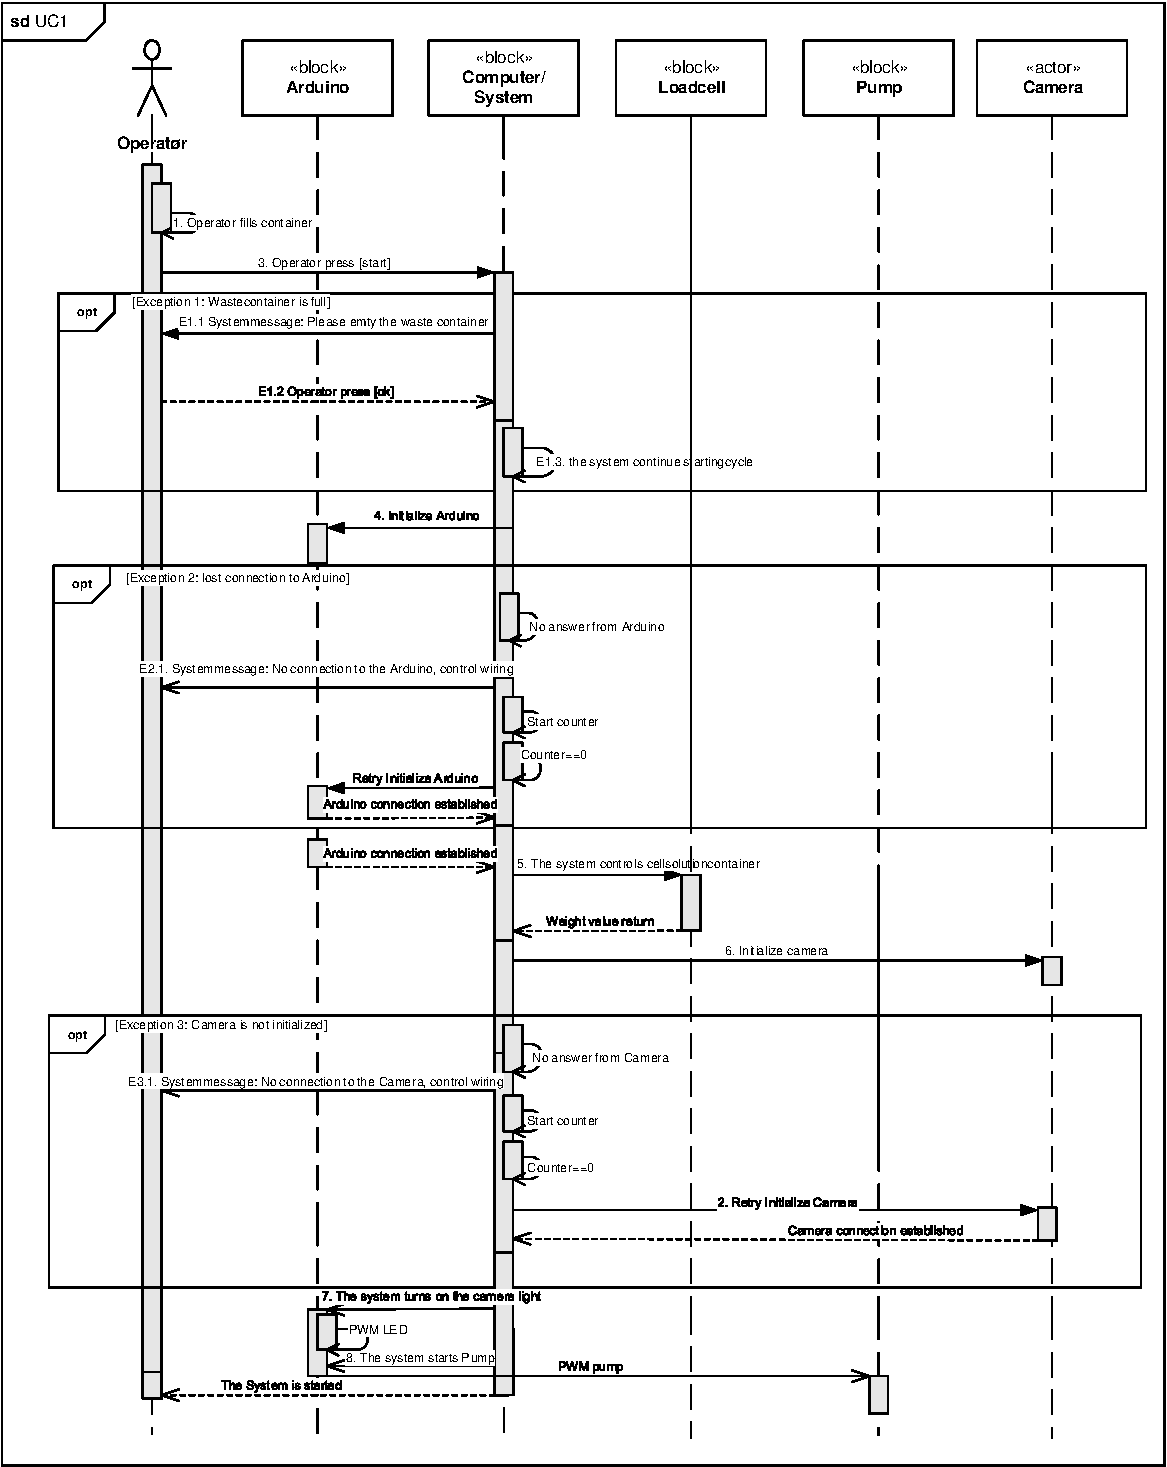
\includegraphics[width=1\textwidth]{pdf/UC1_cropped.pdf}
	\caption{Sekvensdiagram for usecase 1}
	\label{fig:sekvendisgr}
\end{figure}


\section{Implementering og enhedstest}
\label{subsec:Implement}
I dette afsnit er der vist et eksempel på hvordan delene er implementeret ved at vise vægtcellen for både hardware og software.

\subsection{Hardware}
afventer samuel
\subsection{Software}
afventer samuel




\section{Cost-benefit analyse}
Økonomisk






Andre ting?